\documentclass{article}
\usepackage{graphicx}
\usepackage{amsmath}
\usepackage{amsfonts}
\usepackage{float}
\usepackage{hyperref}
\usepackage{listings}
\usepackage{xcolor}
\usepackage{geometry}
\usepackage{subcaption}
\geometry{a4paper, margin=1in}

\definecolor{LinkColor}{rgb}{0, 0, 0.5}
\hypersetup{colorlinks=true, linkcolor=LinkColor, citecolor=LinkColor, filecolor=LinkColor, urlcolor=LinkColor}

\title{\textbf{Analytical Study of Least Squares Methods in Overdetermined Systems}}
\author{Kevin Smith}
\date{\today}

\begin{document}

\maketitle


\section{Introduction}
Overdetermined systems are ubiquitous in fields such as engineering and data science, demanding robust and efficient solution methods. The least squares approaches, particularly their regularized variants, stand out as powerful tools for addressing these challenges. This work investigates their efficacy through computational experiments designed to shed light on the influence of regularization on solution stability and accuracy.

\section{Problem Statement}
The fundamental problem addressed is the minimization of the residual $\|Ax - b\|^2$ for systems where $A \in \mathbb{R}^{n \times k}$ with $n > k$. Such systems commonly lack exact solutions, prompting the need for an approximate solution that can be effectively found via least squares methods. The addition of a regularization term helps to mitigate the effects of noise and errors in the data, ensuring a balanced solution.

\section{Methodology}
\subsection{Implementation Details}
We utilized NumPy within Python for our implementations, benefiting from its efficiency in matrix operations. Our methodology involved the application of Householder transformations for QR decomposition, enabling us to convert complex systems into a more manageable upper triangular form. We also explored an incremental updating algorithm suitable for dynamic data processing.

\subsection{Test Design}
The testing protocol involved synthetic datasets with known solutions and covered a range of problem sizes. This allowed us to thoroughly assess the scalability of the algorithms and their robustness in both consistent and inconsistent system conditions.

\section{Results and Discussion}

\subsection{Accuracy and Statistical Behavior}
Comparative analysis of the traditional batch method and the incremental least squares method revealed a remarkable consistency in performance. The incremental least squares method, in particular, is designed to update the solution as new data points are added to the system, making it well-suited for real-time applications where data arrives sequentially. As visualized in the error plots presented in Figure \ref{fig:error_plots}, both methods exhibit stable performance with the error remaining within acceptable bounds across varying problem sizes. This stability is a testament to the robustness of the least squares approach in handling systems of different scales without significant loss of accuracy.

\begin{figure*}[t!]
    \centering
    \caption{Relative error and condition number analyses for the incremental and traditional least squares methods, highlighting the algorithms' performance across varying problem sizes.}
    \label{fig:error_plots}
    \begin{subfigure}[b]{.45\textwidth}
        \centering
        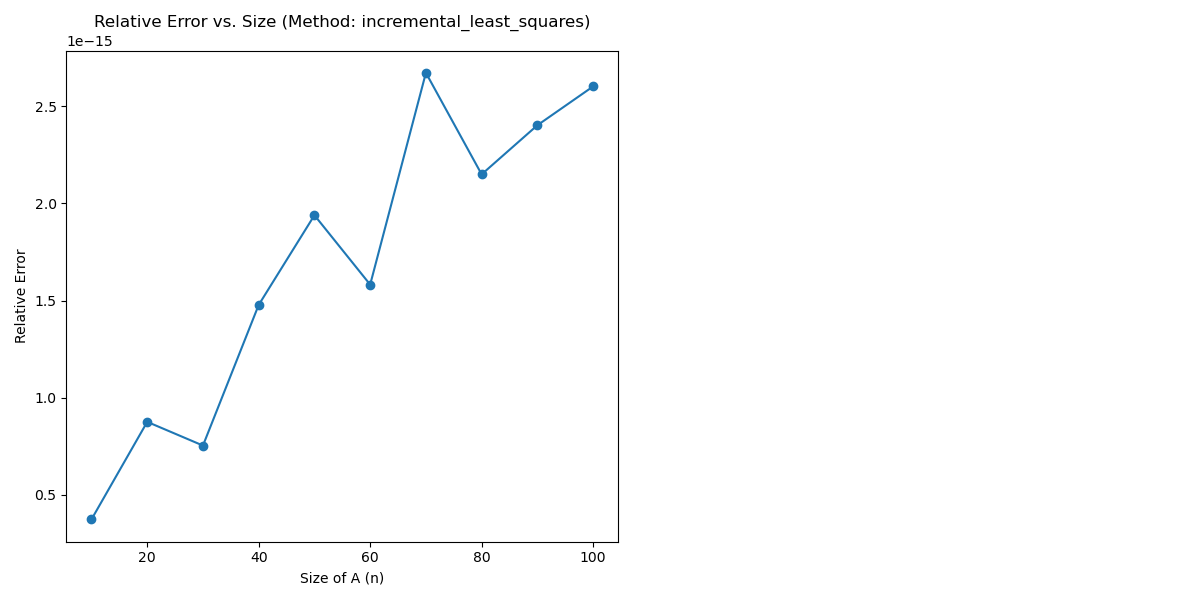
\includegraphics[width=\linewidth]{errorplot_incremental_least_squares.png}
        \caption{Relative error vs. problem size for the incremental least squares method.}
        \label{fig:error_incremental}
    \end{subfigure}
    ~ % This adds a little space between figures
    \begin{subfigure}[b]{.45\textwidth}
        \centering
        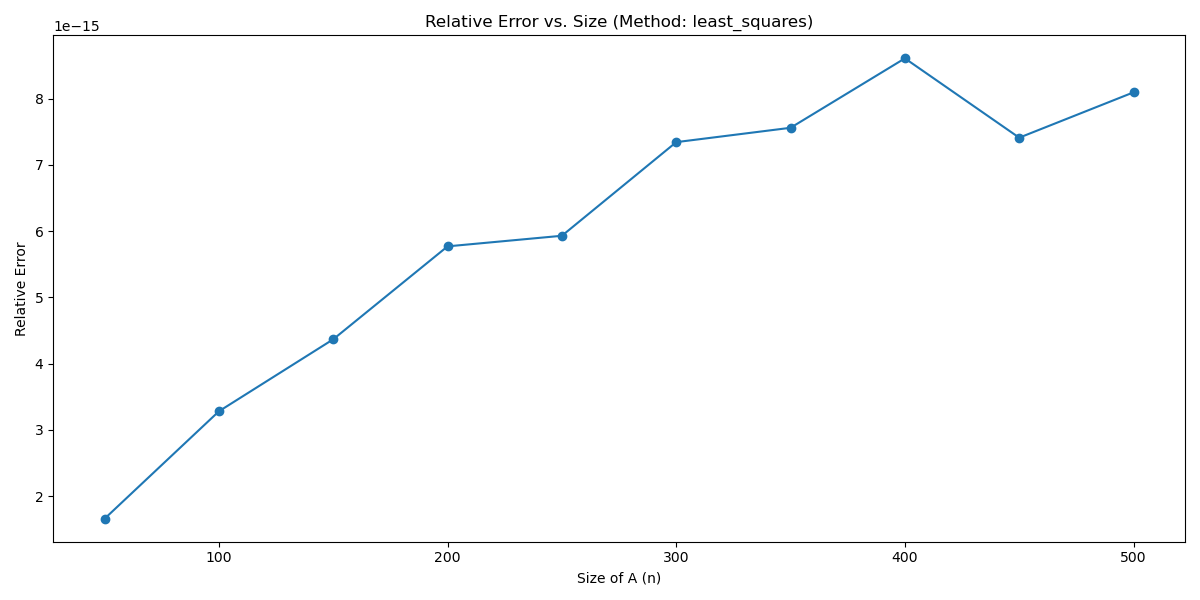
\includegraphics[width=\linewidth]{errorplot_least_squares.png}
        \caption{Relative error vs. problem size for the traditional least squares method.}
        \label{fig:error_least_squares}
    \end{subfigure}
\end{figure*}

The relative error plots provide insight into the accuracy of the least squares methods as the problem size increases. As observed in Figure \ref{fig:error_plots}, both the incremental and traditional methods exhibit stable performance with the error remaining within acceptable bounds. This indicates the robustness of the least squares approach in handling systems of varying sizes without significant loss of accuracy.



\subsection{Impact of Regularization}
The critical role of regularization is exemplified in the signal reconstruction plots provided in Figure \ref{fig:signal_reconstructions}, where the choice of $\lambda$ significantly influenced the trade-off between noise reduction and the preservation of signal integrity.

\begin{figure*}[t!]
    \centering
    \caption{Signal reconstructions for different regularization parameters compared with the true signal, demonstrating the effect of varying $\lambda$ values on signal fidelity.}
    \label{fig:signal_reconstructions}
    % First row with two images
    \begin{subfigure}[t]{0.5\textwidth}
        \centering
        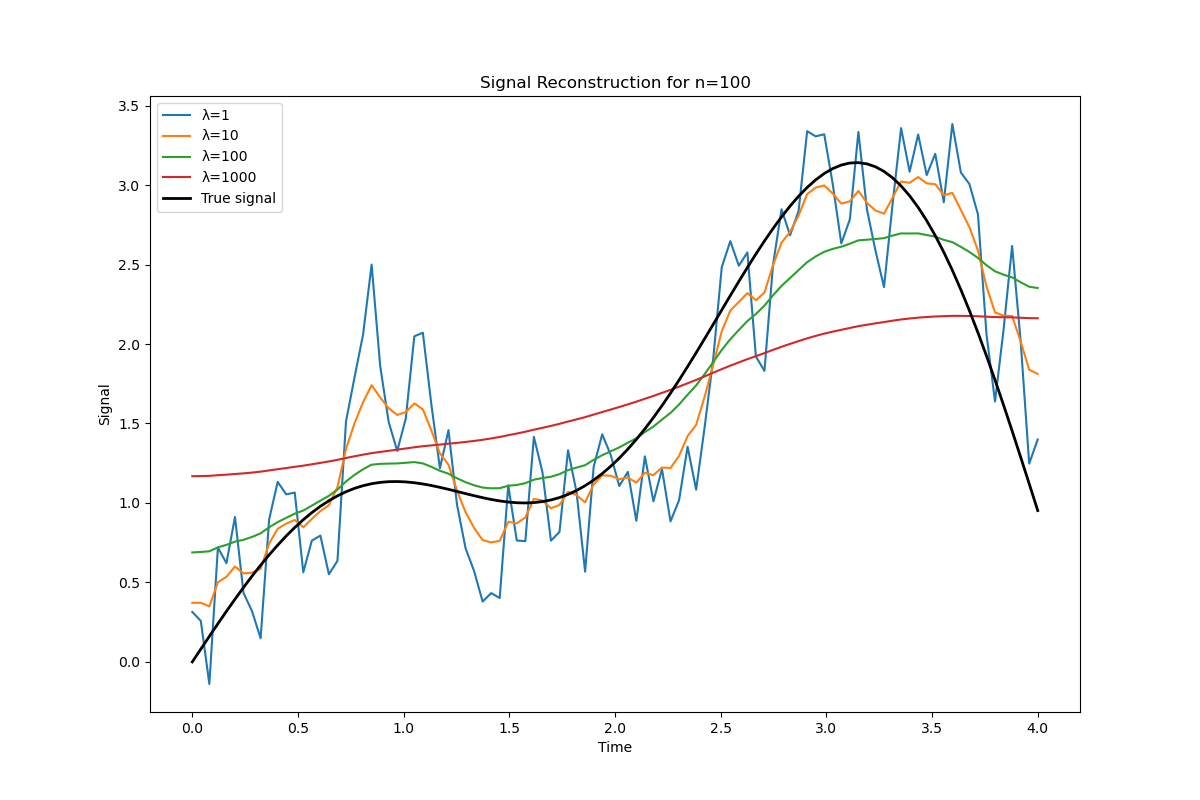
\includegraphics[height=2.0in]{signalplot_100.png}
        \caption{Signal reconstruction for $n=100$.}
        \label{fig:signal100}
    \end{subfigure}%
    ~ % This adds a little space and allows the figures to be side by side
    \begin{subfigure}[t]{0.5\textwidth}
        \centering
        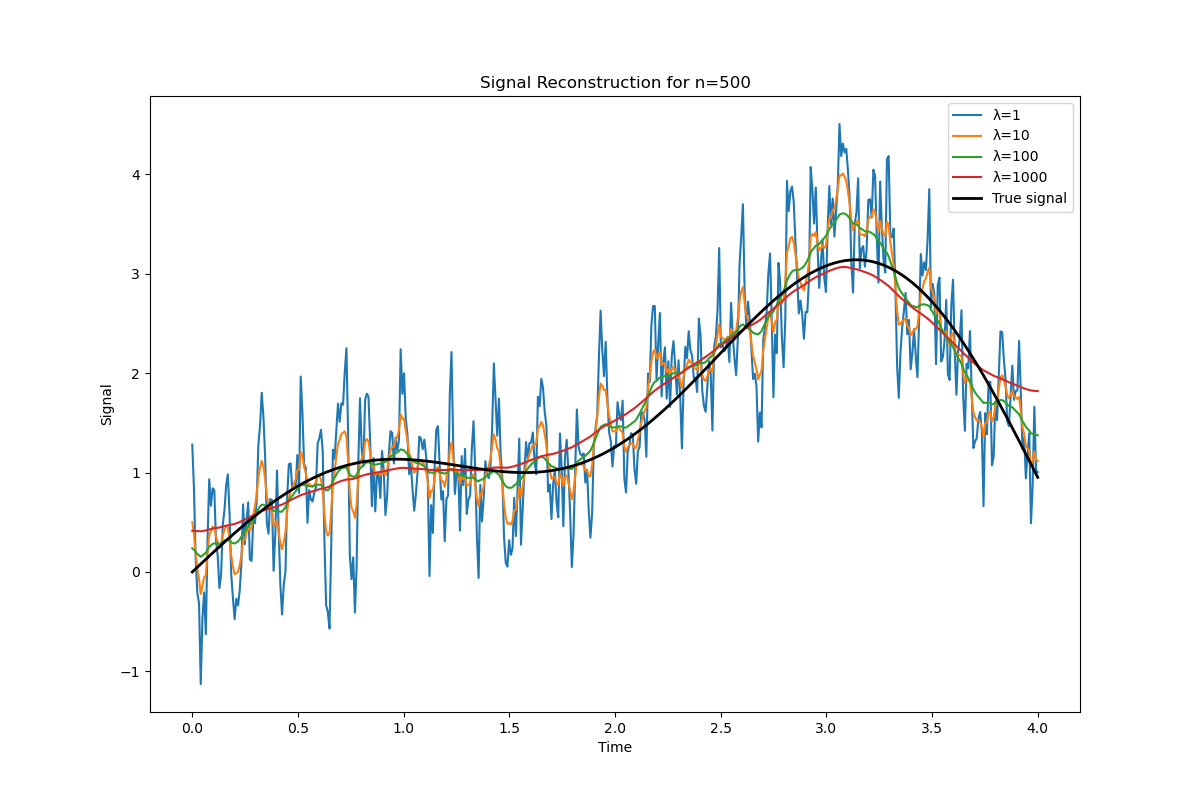
\includegraphics[height=2.0in]{signalplot_500.png}
        \caption{Signal reconstruction for $n=500$.}
        \label{fig:signal500}
    \end{subfigure}

\end{figure*}


The results underscore the nuanced balance required in selecting $\lambda$, with implications for real-time applications where the incremental method's efficiency is particularly advantageous.

\section{Conclusion}
The findings affirm the utility of least squares methods in treating overdetermined systems, with regularization serving as a key component for managing the interplay between error minimization and noise suppression. The insights gained point to promising directions for future research, including the development of adaptive regularization techniques and advanced incremental algorithms for high-dimensional problems.

\section{Discussion}
The choice of the regularization parameter $\lambda$ emerges as a critical factor in the effectiveness of the least squares solutions. While too small a $\lambda$ leaves the solution vulnerable to noise, an excessively large $\lambda$ may oversmooth the solution, erasing details in the data. The incremental method is especially promising for dynamic systems where the computational cost of re-solving the entire problem for every new data point is prohibitive.


\end{document}
